\documentclass[10pts]{beamer}
\usepackage[utf8]{inputenc}


\usepackage{multirow,rotating}
\usepackage{color}
\usepackage{hyperref}
\usepackage{tikz-cd}
\usepackage{array}
\usepackage{siunitx}
\usepackage{mathtools,nccmath}%
\usepackage{etoolbox, xparse} 
\usetheme{CambridgeUS}
\usecolortheme{dolphin}
\usepackage{listings}
\usepackage{amsmath}

\DeclarePairedDelimiter\abs{\lvert}{\rvert}%
\DeclarePairedDelimiter\norm{\lVert}{\rVert}%
\makeatletter
\let\oldabs\abs
\def\abs{\@ifstar{\oldabs}{\oldabs*}}
%
\let\oldnorm\norm
\def\norm{\@ifstar{\oldnorm}{\oldnorm*}}
\makeatother


% set colors
\definecolor{myNewColorA}{RGB}{158, 27,50}
\definecolor{myNewColorB}{RGB}{158, 27,50}
\definecolor{myNewColorC}{RGB}{158, 27,50} % {130,138,143}
\setbeamercolor*{palette primary}{bg=myNewColorC}
\setbeamercolor*{palette secondary}{bg=myNewColorB, fg = white}
\setbeamercolor*{palette tertiary}{bg=myNewColorA, fg = white}
\setbeamercolor*{titlelike}{fg=myNewColorA}
\setbeamercolor*{title}{bg=myNewColorA, fg = white}
\setbeamercolor*{item}{fg=myNewColorA}
\setbeamercolor*{caption name}{fg=myNewColorA}
\usefonttheme{professionalfonts}
\usepackage{natbib}
\usepackage{hyperref}




\definecolor{white}{rgb}{1.0, 1.0, 1.0}
\definecolor{codegray}{rgb}{0.5,0.5,0.5}
\definecolor{codepurple}{rgb}{0.58,0,0.82}
\definecolor{codegreen}{rgb}{0,0.6,0}
%------------------------------------------------------------
% \titlegraphic{
\includegraphics[height=0.75cm]{uni-logo.png}} 

% logo of my university


\title{Dirigida 2}

\author[]{Malvaceda Canales Carlos Daniel$^1$ \and Huanca Contreras Henry$^{19}$ \and Catalino Morales Breiner$^{17}$ \and Cipriano Arroyo Bruno$^3$
}
\title{Dirigida 2\\CM4F1 - Análisis y Modelamiento Numérico \\Pregunta 1,3,17,19}
\date{15 de Octubre del 2022}

\begin{document}

\maketitle

\section{Pregunta 1}

\begin{frame}{Pregunta 1}
     Obtenga los números de condición relativos de las siguientes funciones :

        \begin{equation}
        \begin{split}
	    &a) \ f(x)=x^p \\
	    &b) \ f(x)=log(x) \\
	    &c) \ f(x)=cos(x) \\
	    &d) \ f(x)=e^x
	    \end{split}
        \end{equation}
        
\end{frame}

\begin{frame}{Solución}
    
        \begin{block}{Definición}
		El número de condición relativo $\kappa = \kappa(x)$ del problema $f$ en $x$ es 
		\[ \kappa = \lim_{\delta\to 0} \sup_{\ |h|<\delta} \Bigg | \frac{\frac{\ df(x;h)}{f(x)}}{\frac{h}{x}} \Bigg |\ \]
	\end{block}
	
	Si $f$ es diferenciable $\kappa = \bigg | \frac{x f'(x)}{f(x)} \bigg|$
	
	
    
\end{frame}

\vspace*{\fill}
Para $f(x) = x^p$ calculamos el número de condición relativo 

    \[ \ f(x)=x^p\]
    \[ \ f'(x)= px^{p-1} \]
    \[\kappa = \bigg | \frac{x f'(x)}{f(x)} \bigg|  = \bigg | \frac{x.p .x^{p-1}}{x^p} \bigg| = |p| < 1\]
    \[\Rightarrow -1<p<1	 \]
    Por lo tanto para valores de  $p \in \langle -1,1\rangle$ , el problema estará bien condicionado.

\vspace*{\fill}

\newpage

\vspace*{\fill}

Para $f(x) = \log(x)$ calculamos el número de condición relativo

    \[\kappa = \Bigg| \frac{x}{(x\ln{10})\log{x} }\Bigg|\]
    \[\kappa = \Bigg| \frac{1}{\ln{10}\log{x} }\Bigg| < 1\]
    \[-1<\frac{1}{\ln{10}\log{x} } <1\]
    \[-1<\frac{1}{\ln{10}\log{x} }\]
    \[\Rightarrow   (0<x<\frac{1}{10^{\frac{1}{\ln(10)}}}) \lor (x>1)\]
    

\vspace*{\fill}
%
\newpage

\vspace*{\fill}

    
    \[\frac{1}{\ln{10}\log{x} } <1\]
    \[\frac{1}{\ln{10} } <\log{x}\]
    \[\Rightarrow (0<x<1) \lor (x > 10^{\frac{1}{\ln(10)}})\]
    Por lo tanto para valores de $x$
    \[  ((0<x<\frac{1}{10^{\frac{1}{\ln(10)}}}) \lor (x>1))  \land ((0<x<1) \lor (x > 10^{\frac{1}{\ln(10)}}))\]
    \[\Rightarrow x \in \langle 0,\frac{1}{10^{\frac{1}{\ln(10)}}}\rangle \cup \langle 10^{\frac{1}{\ln(10)}},\infty\rangle\]
    el problema estará bien condicionado.
    
\vspace*{\fill}
%

\newpage
\vspace*{\fill}

Para $f(x) = \cos{x}$ calculamos el número de condición relativo
\[\kappa = \Bigg| \frac{x(-\sin{x})}{\cos{x}} \Bigg|\]
\[\kappa = |-x \tan x |=|x \tan x |<1\]
Usando la aproximación de Maclaurin-Taylor alrededor del $x=0$
\[\tan(x) = x + \frac{1}{3}x^3+\frac{2}{15^2}x^5+...\]
Utilizando esos 3 valores como referencia
\[\kappa= \big|(-x)(x + \frac{1}{3}x^3+\frac{2}{15^2}x^5)\big|\]


\vspace*{\fill}
\newpage
\vspace*{\fill}

\[\kappa= \big|x(x + \frac{1}{3}x^3+\frac{2}{15^2}x^5)\big|\]
\[\kappa= \big|x^2+\frac{1}{3}x^4+\frac{2}{15^2}x^6\big|<1\]
\[x^2+\frac{1}{3}x^4+\frac{2}{15^2}x^6<1\]
Por lo tanto para valores de $x$ , tal que 
\[ x \in \langle -0.888,0.888 \rangle \]
el problema estará bien condicionado.

\vspace*{\fill}


\newpage
\vspace*{\fill}
Para $f(x) = e^x$ calculamos el número de condición relativo
\[f(x)=e^x\]
\[f'(x)=e^x\]
\[\kappa = \Bigg| \frac{x.e^x}{e^x} \Bigg|<1\]
\[-1<x<1\]
Por lo tanto para valores de $x$ , tal que $x \in \langle -1,1 \rangle$ el problema estará bien condicionado.

\vspace*{\fill}
\newpage



 %-------------------------------------------% 
\section{Pregunta 3}
%BRUNO 
\begin{frame}{Pregunta 3}
     Obtenga los números de condición relativos de las siguientes funciones :

        \begin{equation}
        \begin{split}
	    &a) \ f(x)=\sqrt{x+5} \\
	    &b) \ f(x)=cos(2{\pi}x) \\
	    &c) \ f(x)=e^{-x^2} 
	    \end{split}
        \end{equation}
        
\end{frame}

\begin{frame}{Solución}

\vspace*{\fill}
Para $f(x) = \sqrt{x+5}$ calculamos el número de condición relativo 

    \[ \ f(x)=\sqrt{x+5}\]
    \[ \ f'(x)= \frac{1}{2\sqrt{x+5}} \]
    \[\kappa = \bigg | \frac{x f'(x)}{f(x)} \bigg|  = \bigg | \frac{x.\frac{1}{2\sqrt{x+5}}}{\sqrt{x+5}} \bigg| = \bigg|\frac{1}{2}-\frac{5}{2(x+5)}\bigg| < 1\]
    \[ \ \frac{-1}{2}<\frac{5}{2(x+5)}<\frac{3}{2}\]
    \[ \ \frac{-1}{2}<\frac{5}{2(x+5)} \land \frac{5}{2(x+5)}<\frac{3}{2}\]
    \[ \ -10<x \land \frac{-10}{3}<x\]
    Por lo tanto para valores de  $x \in \langle \frac{-10}{3},\infty\rangle$ , el problema estará bien condicionado.
\vspace*{\fill}
\end{frame}

\newpage
\begin{frame}{Solución}
\vspace*{\fill}
Para $f(x)=cos(2{\pi}x)$ calculamos el número de condición relativo 

    \[ \ f(x)=cos(2{\pi}x)\]
    \[ \ f'(x)= -2{\pi}sen(2{\pi}x) \]
    \[\kappa = \bigg | \frac{-2x{\pi}sen(2{\pi}x)}{cos(2{\pi}x)} \bigg|  = \bigg | -2{\pi}xtan(2{\pi}x) \bigg| < 1\]
    \[ \Rightarrow \frac{arctan(\frac{-1}{2\pi})}{2\pi}<x<\frac{arctan(\frac{1}{2\pi})}{2\pi}\]
    Por lo tanto para valores de  $x \in \langle -1.4392478714108,1.4392478714108\rangle$ , el problema estará bien condicionado.
\vspace*{\fill}
\end{frame}
\newpage
\begin{frame}{Solución}
Para $f(x) = e^{-x^2}$ calculamos el número de condición relativo 

    \[ \ f(x)=e^{-x^2}\]
    \[ \ f'(x)= -2e^{-x^2} \]
    \[\kappa = \bigg | \frac{-2x^2e^{-x^2}}{e^{-x^2}} \bigg|  = |-2x^2| = |2x^2| < 1\]
    \[\Rightarrow 0<x<\sqrt{\frac{1}{2}}\]
    Por lo tanto para valores de  $x \in \langle 0,\sqrt{\frac{1}{2}}\rangle$ , el problema estará bien condicionado.
\vspace*{\fill}
\end{frame}
%-------------------------------------------%

%Catalino
\section{Pregunta 17}


\begin{frame}{Pregunta 17}
El peri\'metro de un recta\'ngulo es 64 cm y la diferencia entre las medidas de la base y la altura es 6
cm. Determine las dimensiones de dicho recta\'ngulo.
\vspace{0.2 cm}\\
a) Modele el problema.\\
sean los lados:\\
a:altura \\
b:base\\
\vspace{0.2 cm}
Ecuaciones \hspace{3cm} Ordenando las ecuaciones\\
2b+2a=64 \hspace{3cm} b+a=32\\
b-a=6 \hspace{3.76cm}  b-a=6\\
\vspace{0.5 cm}

\end{frame}
\begin{frame}
Matriz A \hspace{3cm} Matriz aumentada\\
\vspace{0.5 cm}
A= \left (
\begin{array}{rr}
1 & 1  \\
1 & -1  \\
\end{array}
\right )
\hspace{2cm}
A|B=\left (
\begin{array}{rr|r}
1 & 1  & 32\\
1 & -1  & 6\\
\end{array}
\right )

\end{frame}

\begin{frame}{}
b) Determine la norma matricial de A y A^{-1}\\
Primero calculamos la inversa de A\\
\vfill
A^{-1} = \frac{adj(A^{t})} {\abs{A} }
\vfill
A^{t}=\left (
\begin{array}{rr}
1 & 1 \\
1 & -1 \\
\end{array}
\right )\hspace{0.5cm}
adj(A^{t})=\left (
\begin{array}{rr}
-1 & -1 \\
-1 & 1 \\
\end{array}
\right )\hspace{0.5cm}
\vspace{0.5 cm}
\abs{A}=-2
\vfill
A^{-1} = \frac{1}{2}\left(
\begin{array}{rr}
-1 & -1 \\
-1 & 1 \\
\end{array}
\right )\hspace{0.5cm}
A^{-1} =\left(
\begin{array}{rr}
 \frac{1}{2}\vspace{0.01 cm} &  \frac{1}{2}\vspace{0.01 cm} \\
 \frac{1}{2}\vspace{0.01 cm} &  -\frac{1}{2}\vspace{0.01 cm}\\
\end{array}
\right )\hspace{0.5cm}\\
\vspace{0.5 cm}

\end{frame}

\begin{frame}{}
Las normas se calculan de la siguiente manera
\vfill
\norm{ A }_p= max_{x \not =0}
 \left\frac{\norm{ AX }_p}{\norm{ X }_p} \right\\
\norm{ A }_1 = max_{1\leq j \leq n} 
\sum_{i=1}^{m}|a_{ij}|\\
\norm{ A }_\infty = max_{1\leq i \leq n}  
\sum_{j=1}^{n}|a_{ij}|\\
\begin{equation*}\\
Para la matriz A\\
Fila 1:\abs{1} + \abs{1} =2\\
Fila 2:\abs{1} + \abs{-1} =2\\
Columna 1:\abs{1} + \abs{1}=2\\
Columna 2:\abs{1} + \abs{-1}=2\\
\norm{ A }_1=\max(2,2) =2\hspace{0.5cm}
\norm{ A }_\infty=\max(2,2) =2
\end{equation*}

\end{frame}
\begin{frame}{}
\begin{equation*}\\
Para la matriz A^{-1}\\
Fila 1:\abs{\frac{1}{2}}+ \abs{\frac{1}{2}}=1\vspace{0.1 cm}\\
Fila 2:\abs{\frac{1}{2}}+ \abs{-\frac{1}{2}}=1\vspace{0.1 cm} \\
Columna 1:\abs{\frac{1}{2}}+ \abs{\frac{1}{2}}=1\vspace{0.1 cm} \\
Columna 2:\abs{\frac{1}{2}}+ \abs{-\frac{1}{2}}=1\vspace{0.1 cm} \\
\norm{ A^{-1} }_1=\max(1,1) =1\hspace{0.5cm}
\norm{ A^{-1} }_\infty=\max(1,1) =1
\end{equation*}

\end{frame}

\begin{frame}{}
c) Determine la soluci\'on usando los m\'etodos de Gauss y Gauss-Jordan.\\
\vspace{0.2 cm}
ordenando con pivoteo parcial\\
\vspace{0.2 cm}
\left (
\begin{array}{rr|r}
1 & 1 &32\\
1 & -1 &6
\end{array}
\right )\\
\vspace{0.2 cm}

\end{frame}

\begin{frame}
1) metod\'o de gauss\\
\vspace{0.5 cm}
\xrightarrow{F_2 = F_2-F_1}\left (
\begin{array}{rr|r}
1 & 1  & 32\\
0 & -2  & -26
\end{array}
\right )\hspace{1cm}
\vspace{0.2 cm}
\begin{equation*}\\
entonces:\\
    -2a&=-26,\hspace{1cm}a&=13\\
    b+a&=32,\hspace{1cm}b&=19\\
\end{equation*}
la base b=19\\
la altura a=13

\end{frame}
\begin{frame}{}
\begin{figure}
    \centering
    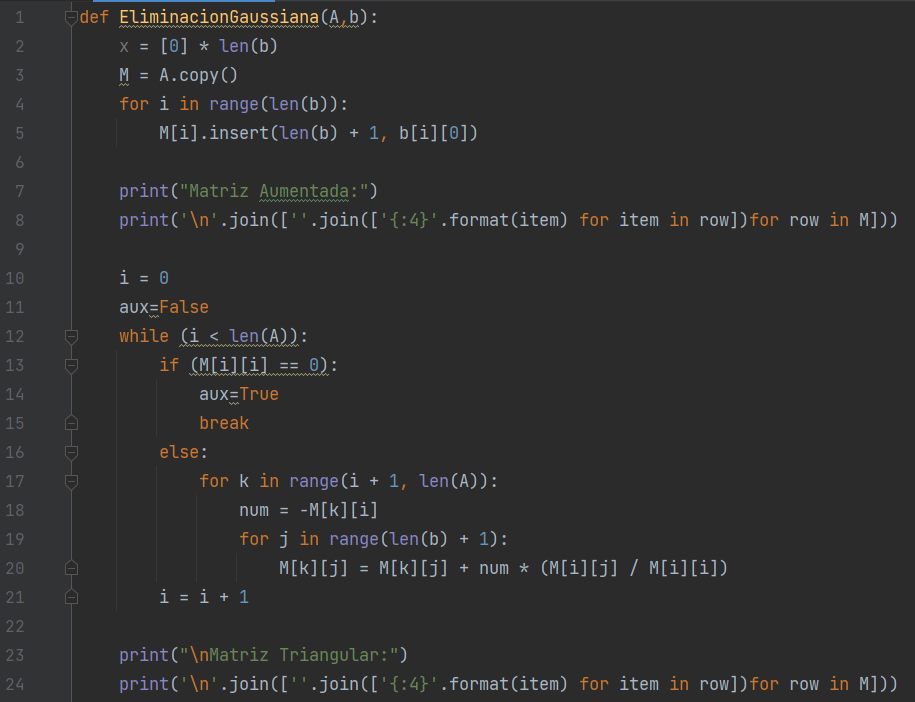
\includegraphics[scale=0.44]{17-GAUSS-PARTE1.PNG}
\end{figure}
\end{frame}
\begin{frame}{}
\begin{figure}
    \centering
    
\includegraphics[scale=0.44]{17-GAUSS-PARTE2.PNG}
\end{figure}
\end{frame}
\begin{frame}{}
\begin{figure}
    \centering
    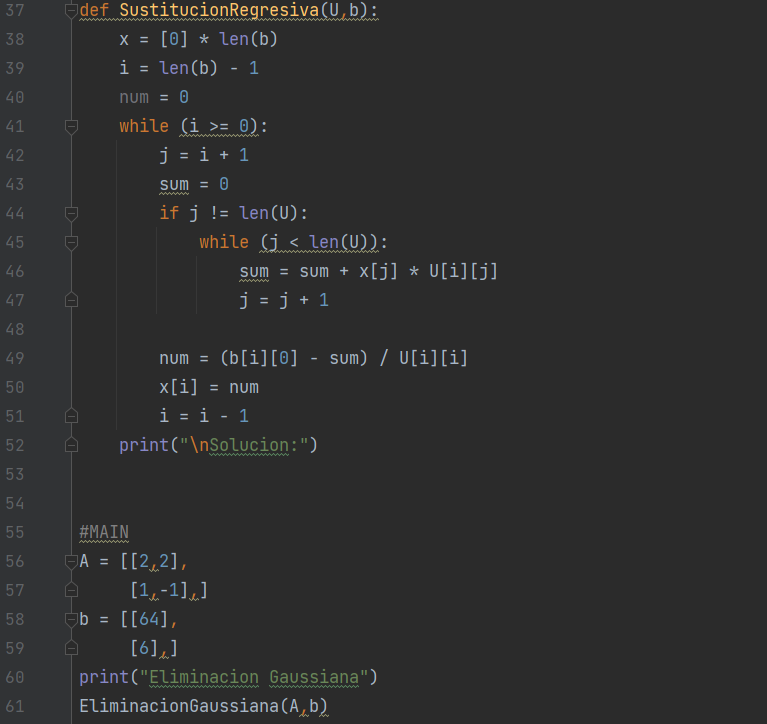
\includegraphics[scale=0.44]{17-GAUSS-PARTE3.PNG}
\end{figure}
\end{frame}
\begin{frame}{}
\begin{figure}
    \centering
    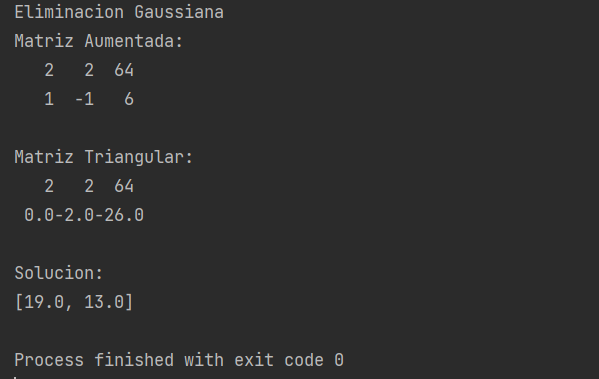
\includegraphics[scale=0.44]{17-GAUSS-PARTE4.PNG}
\end{figure}
\end{frame}

\begin{frame}{}
2) metod\'o de gauss-jordan\\
\vspace{0.5 cm}
\xrightarrow{F_2 = F_2-F_1}\left (
\begin{array}{rr|r}
1 & 1  & 32\\
0 & -2  & -26
\end{array}
\right )\hspace{1cm}
\vspace{0.2 cm}\\
\xrightarrow{F_2 = \frac{F_2}{-2}}\left (
\begin{array}{rr|r}
1 & 1  & 32\\
0 & 1  & 13
\end{array}
\right )\hspace{1cm}
\vspace{0.2 cm}\\
\xrightarrow{F_1 = F_1-F_2}\left (
\begin{array}{rr|r}
1 & 0  & 19\\
0 & 1  & 13
\end{array}
\right )\hspace{1cm}
\vspace{0.2 cm}
\begin{equation*}\\
entonces:\\
    b\hspace{0.5 cm}&=19\\
    \hspace{0.5 cm}a\hspace{0.1 cm}&=13\\
\end{equation*}
la base b=19\\
la altura a=13

\end{frame}
\begin{frame}{}
\begin{figure}
    \centering
    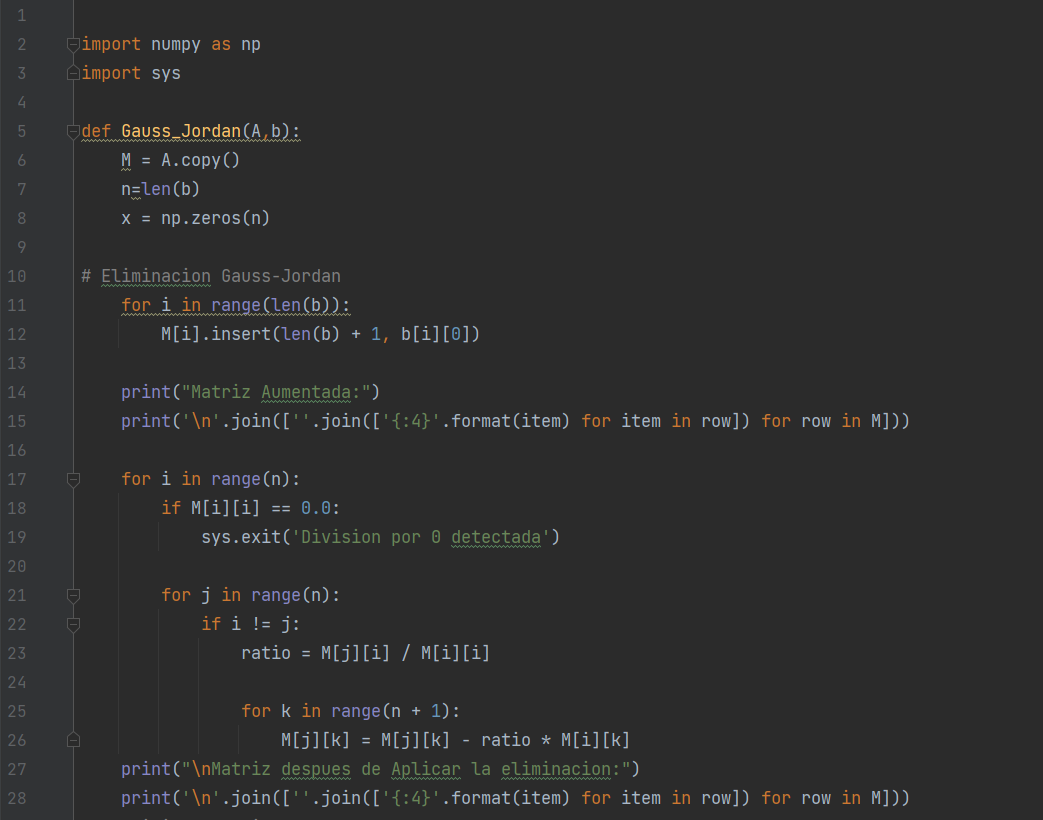
\includegraphics[scale=0.33]{17-GAUSS-JORDAN-PARTE1.PNG}
\end{figure}
\end{frame}

\begin{frame}{}
\begin{figure}
    \centering
    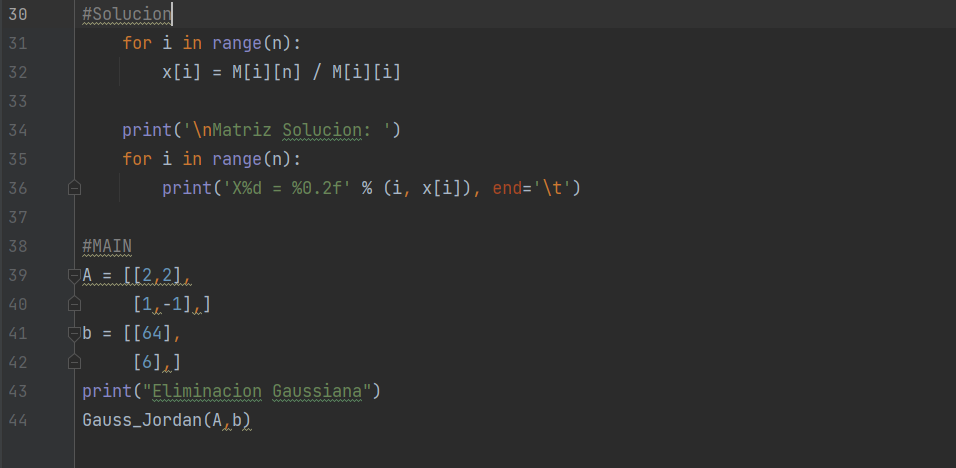
\includegraphics[scale=0.44]{17-GAUSS-JORDAN-PARTE2.PNG}
\end{figure}
\end{frame}
\begin{frame}{}
\begin{figure}
    \centering
    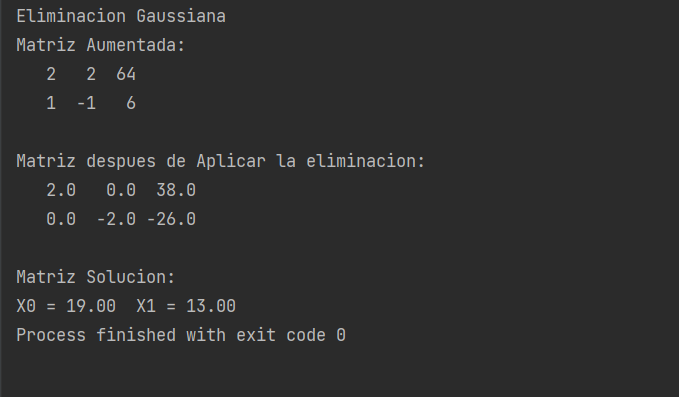
\includegraphics[scale=0.44]{17-GAUSS-JORDAN-PARTE3.PNG}
\end{figure}
\end{frame}



%-------------------------------------------%






\section{Pregunta 19}


\begin{frame}{Pregunta 19}
Se juntan 30 personas entre hombres, mujeres y ni\~{n}os. Se sabe que entre los hombres y las mujeres
duplican al n\'umero de ni\~{n}os. Tambi\'en se sabe que entre los hombres y el triple de las mujeres
exceden en 20 al doble de ni\~{n}os.\\
\vspace{0.2 cm}
a) Modele el problema.\\
x:hombres\\
y:mujeres\\
z:ni\~{n}os\\
\vspace{0.2 cm}
Ecuaciones \hspace{3cm} ordenando las ecuaciones\\
x+y+z=30 \hspace{3cm} x+y+z=30\\
x+y=2z \hspace{3.5cm} x+y-2z=0\\
x+3y=2z+20 \hspace{2.7cm} x+3y-2z=20\\
\vspace{0.5 cm}

\end{frame}
\begin{frame}
Matriz A \hspace{3cm} Matriz aumentada\\
\vspace{0.5 cm}
A= \left (
\begin{array}{rrr}
1 & 1 & 1 \\
1 & 1 & -2 \\
1 & 3 & -2
\end{array}
\right )
\hspace{2cm}
A|B=\left (
\begin{array}{rrr|r}
1 & 1 & 1 & 30\\
1 & 1 & -2 & 0\\
1 & 3 & -2 & 20
\end{array}
\right )

\end{frame}

\begin{frame}{}
b) Determine la norma matricial de A y A^{-1}\\
\vspace{0.5 cm}
\left (
\begin{array}{rrr|rrr}
1 & 1 & 1 & 1 & 0 &0\\
1 & 1 & -2 & 0 & 1 &0\\
1 & 3 & -2 & 0 & 0 &1
\end{array}
\right )\hspace{0.5cm}
\left (
\begin{array}{rrr|rrr}
1 & 1 & 1 & 1 & 0 &0\\
1 & 3 & -2 & 0 & 0 &1\\
1 & 1 & -2 & 0 & 1 &0
\end{array}
\right )\\
\vspace{0.5 cm}
\left (
\begin{array}{rrr|rrr}
1 & 1 & 1 & 1 & 0 &0\\
1 & 3 & -2 & 0 & 0 &1\\
0 & 0 & -3 & -1 & 1 &0
\end{array}
\right )\hspace{0.5cm}
\left (
\begin{array}{rrr|rrr}
1 & 1 & 1 & 1 & 0 &0\\
0 & 2 & -3 & -1 & 0 &1\\
0 & 0 & -3 & -1 & 1 &0
\end{array}
\right )\\
\vspace{0.5 cm}
\left (
\begin{array}{rrr|rrr}
1& 1 & 1 & 1 & 0 &0\\
0 & 2 & -3 & -1 & 0 &1\\
0 & 0 & 1 & 1/3 & -1/3 &0
\end{array}
\right )
\left (
\begin{array}{rrr|rrr}
1& 1 & 1 & 1 & 0 &0\\
0 & 2 & 0 & 0 & -1 &1\\
0 & 0 & 1 & 1/3 & -1/3 &0
\end{array}
\right )
\end{frame}
\begin{frame}{}
\left (
\begin{array}{rrr|rrr}
1& 1 & 0 & 2/3 & 1/3 &0\\
0 & 2 & 0 & 0 & -1 &1\\
0 & 0 & 1 & 1/3 & -1/3 &0
\end{array}
\right )\hspace{0.5cm}
\left (
\begin{array}{rrr|rrr}
1& 1 & 0 & 2/3 & 1/3 &0\\
0 & 1 & 0 & 0 & -1/2 &1/2\\
0 & 0 & 1 & 1/3 & -1/3 &0
\end{array}
\right )\\
\vspace{0.5 cm}
\left (
\begin{array}{rrr|rrr}
1& 0 & 0 & 2/3 & 5/6 &-1/2\\
0 & 1 & 0 & 0 & -1/2 &1/2\\
0 & 0 & 1 & 1/3 & -1/3 &0
\end{array}
\right ) \hspace{0.5cm}
A^{-1}=\left (
\begin{array}{rrr}
2/3 & 5/6 &-1/2\\
0& -1/2 &1/2\\
1/3 & -1/3 &0
\end{array}
\right ) \\
\vspace{0.5 cm}
\end{frame}
\begin{frame}{}
\norm{ A }_p= max_{x \not =0}
 \left\frac{\norm{ AX }_p}{\norm{ X }_p} \right\\
\norm{ A }_1 = max_{1\leq j \leq n} 
\sum_{i=1}^{m}|a_{ij}|\\
\norm{ A }_\infty = max_{1\leq i \leq n}  
\sum_{j=1}^{n}|a_{ij}|\\
para la matriz A\\
\norm{ A }_1=(3,5,5) =5\\
\norm{ A }_\infty=(3,0,2) =3\\
para la matriz A^{-1}\\
\norm{ A^{-1} }_1=(1,0,0) =1\\
\norm{ A^{-1} }_\infty=(1,0,0) =1

\end{frame}
\begin{frame}{}
c) Determine la soluci\'on usando los m\'etodos de Gauss y Gauss-Jordan.\\
\vspace{0.2 cm}
ordenando con pivoteo parcial\\
\vspace{0.2 cm}
\left (
\begin{array}{rrr|r}
1 & 1 & 1 & 30\\
1 & 3 & -2 & 20\\
1 & 1 & -2 & 0
\end{array}
\right )\\
 \vspace{0.2 cm}
 \end{frame}
 \begin{frame}
1) metod\'o de gauss\\
\vspace{0.5 cm}
\xrightarrow{F_2 = F_2-F_1}\left (
\begin{array}{rrr|r}
1 & 1 & 1 & 30\\
0 & 2 & -3 & -10\\
1 & 1 & -2 & 0
\end{array}
\right )\hspace{1cm}
\xrightarrow{F_3 = F_3-F_1}\left (
\begin{array}{rrr|r}
1 & 1 & 1 & 30\\
0 & 2 & -3 & -10\\
0 & 0 & -3 & 0
\end{array}
\right )\\
 \vspace{0.2 cm}
-3z=-30 , z=10\\
2y-3(10)=-10 , y=10\\
x+10+10=30 , x=10\\
Asistieron 10 hombre,10 mujeres y 10 niños
\end{frame}
\begin{frame}{}
\begin{figure}
    \centering
    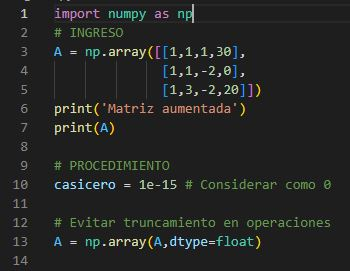
\includegraphics{gauss parte 1.JPG}
\end{figure}
\end{frame}
\begin{frame}{}
\begin{figure}
    \centering
    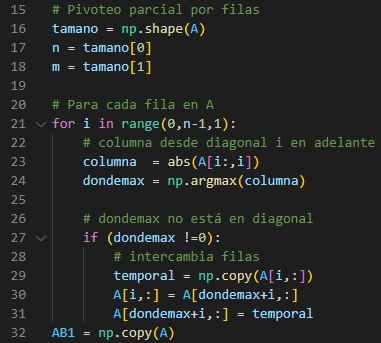
\includegraphics{gauss parte 2.JPG}
\end{figure}
\end{frame}
\begin{frame}{}
\begin{figure}
    \centering
    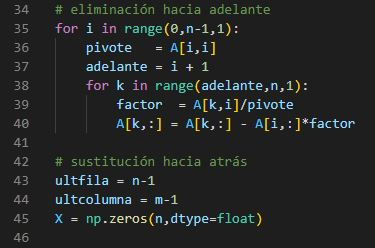
\includegraphics{gauss parte 3.JPG}
\end{figure}
\end{frame}
\begin{frame}{}
\begin{figure}
    \centering
    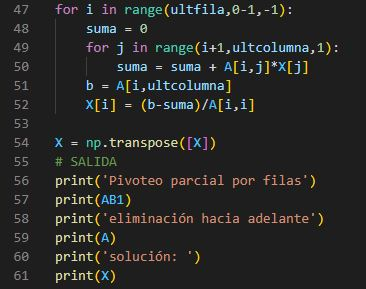
\includegraphics{gauss parte 4.JPG}
\end{figure}
\end{frame}
\begin{frame}{}
\begin{figure}
    \centering
    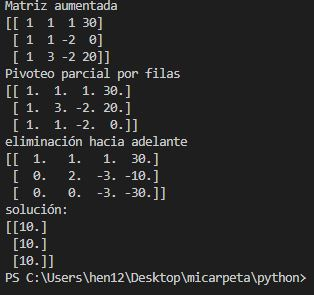
\includegraphics{gauss parte 5.JPG}
\end{figure}
\end{frame}
\begin{frame}{}
2) metod\'o de gauss-jordan\\
\left (
\begin{array}{rrr|r}
1 & 1 & 1 & 30\\
0 & 2 & -3 & -10\\
0 & 0 & -3 & -30
\end{array}
\right ) \hspace{1cm}
\xrightarrow{F_3 = -F_3/3}\left (
\begin{array}{rrr|r}
1 & 1 & 1 & 30\\
0 & 2 & -3 & -10\\
0 & 0 & 1 & 10
\end{array}
\right )\\
 \vspace{0.2 cm}
\xrightarrow{F_2 = F_2+3F_3}\left (
\begin{array}{rrr|r}
1 & 1 & 1 & 30\\
0 & 2 & 0 & 20\\
0 & 0 & 1 & 10
\end{array}
\right )\hspace{1cm}
\xrightarrow{F_1 = F_1-F_3}\left (
\begin{array}{rrr|r}
1 & 1 & 0 & 20\\
0 & 2 & 0 & 20\\
0 & 0 & 1 & 10
\end{array}
\right )\\
 \vspace{0.2 cm}
\xrightarrow{F_2 = F_2/2}\left (
\begin{array}{rrr|r}
1 & 1 & 0 & 20\\
0 & 1 & 0 & 10\\
0 & 0 & 1 & 10
\end{array}
\right )\hspace{0.5cm}
\xrightarrow{F_1 = F_1-F_2}\left (
\begin{array}{rrr|r}
1 & 0 & 0 & 10\\
0 & 1 & 0 & 10\\
0 & 0 & 1 & 10

\end{array}
\right )\\
 \vspace{0.2 cm}
x=10\\
y=10\\
z=10\\
Asistieron 10 hombres, 10 mujeres, 10 niños
\end{frame}
\begin{frame}{}
\begin{figure}
    \centering
    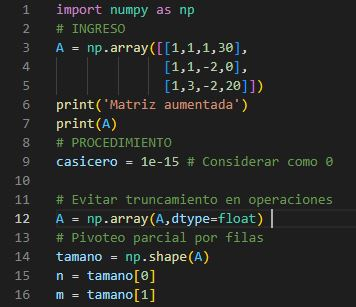
\includegraphics[scale = 0.9]{gauss-jordan parte 1.JPG}
\end{figure}
\end{frame}
\begin{frame}{}
\begin{figure}
    \centering
    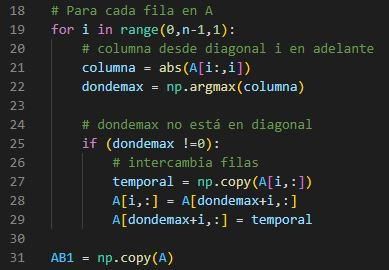
\includegraphics{gauss-jordan parte 2.JPG}
\end{figure}
\end{frame}
\begin{frame}{}
\begin{figure}
    \centering
    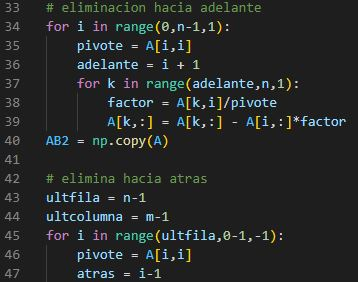
\includegraphics{gauss-jordan parte 3.JPG}
\end{figure}
\end{frame}
\begin{frame}{}
\begin{figure}
    \centering
    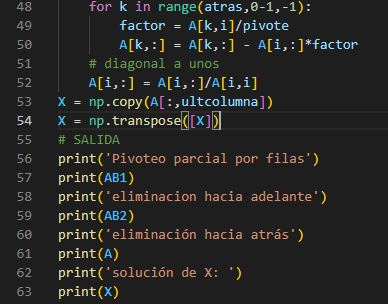
\includegraphics{gauss-jordan parte 4.JPG}
\end{figure}
\end{frame}
\begin{frame}{}
\begin{figure}
    \centering
    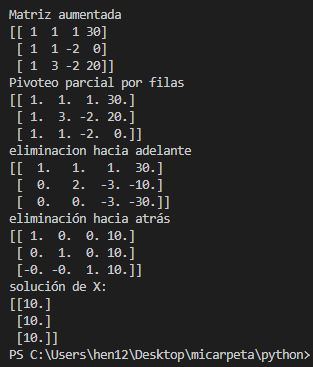
\includegraphics[scale = 0.7]{gauss-jordan parte 5.JPG}
\end{figure}
\end{frame}



	








\end{document}
